%%%%%%%%%%%%%%%%%%%%%%%%%%%%%%%%%%%%%%%%%%%%%%%%%%%%%%%%%%%%%%%%%%%%%%%%%%%%%%%%%%%%%%%%%%%%%%%%%%%
% Chapter 3 -> Methods
% Author: Eduardo G Gusmao
%%%%%%%%%%%%%%%%%%%%%%%%%%%%%%%%%%%%%%%%%%%%%%%%%%%%%%%%%%%%%%%%%%%%%%%%%%%%%%%%%%%%%%%%%%%%%%%%%%%
\chapter{Methods}
\label{cha:methods}

\graphicspath{{chapter3/figs/}}

% Chapter overview
In this chapter we describe the computational footprinting framework we devised to address the problem of active transcription factor binding site identification. Our methodological framework can be divided into two main parts. In the first part, we discuss the input data processing (Section~\ref{sec:input.signal.processing}). We use data from open chromatin NGS-based experiments which gives information regarding the chromatin structure, allowing an accurate search for patterns of active transcription factor binding sites. In this first part we describe all steps involved in the generation of DNase-seq and ChIP-seq signals from the aligned reads and treatment of these signals through several steps which aim at reducing bias and normalizing such genomic signals. In the second part, we define the method we used to identify active transcription factor binding sites (footprints) using the processed signals (Section~\ref{sec:computational.footprinting.hmm}). Such method is based on the probabilistic framework of hidden Markov models (HMMs). Furthermore, we describe some details of the computational implementation of the theory described in this chapter (Section~\ref{sec:implementation}). Finally, we close this chapter with a few concluding remarks on the methodology choice and novelty of our approach (Section~\ref{sec:discussion.3}).

%%%%%%%%%%%%%%%%%%%%%%%%%%%%%%%%%%%%%%%%%%%%%%%%%%%%%%%%%%%%%%%%%%%%%
% Section: Input Signal Processing
%%%%%%%%%%%%%%%%%%%%%%%%%%%%%%%%%%%%%%%%%%%%%%%%%%%%%%%%%%%%%%%%%%%%%
\section{Input Signal Processing}
\label{sec:input.signal.processing}

% Introduction
As mentioned in Section~\ref{sec:current.challenges}, biological data from open chromatin NGS-based experiments, such DNase-seq and ChIP-seq are affected by biases and noises intrinsic to the experimental protocol. Therefore, a number of data processing steps are performed to assuage these biases and noises and also to prepare the data for our computational footprinting method.

% Data as aligned reads
The input data processing pipeline is schematically represented in Figure~\ref{fig:gusmao_signal_pipeline}. In this thesis, we use DNase-seq and histone modification ChIP-seq data as the input for our method. With such data we are able to identify patterns of active transcription factor binding by analyzing the regions in the genome which are both open and protected against DNase I digestion (see Section~\ref{sec:grammar.tfbs}). Our method receives as input the DNase-seq and histone modification ChIP-seq aligned reads (Figure~\ref{fig:gusmao_signal_pipeline}a).

% Count and bias correction
Given the aligned reads, we create genomic signals by counting the overlap between these reads at every genomic coordinate (base pair). This step, which is exemplified in Figure~\ref{fig:gusmao_signal_pipeline}b, is formally shown in Section~\ref{sec:read.overlap.signal}. We refer to this signal as raw genomic signal or read overlap genomic signal. The raw DNase-seq genomic signal is affected by the DNase I sequence cleavage bias. Such bias stems from the fact that the DNase I enzyme prefers to bind to, and cleave, certain genomic sequences. Given that, we perform a DNase-seq sequence cleavage bias correction. The DNase-seq sequence cleavage bias correction, exemplified in Figure~\ref{fig:gusmao_signal_pipeline}c, is thoroughly defined in Section~\ref{sec:dnaseseq.sequence.cleavage.bias}. This step performs local corrections in the DNase-seq signal while preserving signal scale, magnitude and shape.

% Normalization
Both bias-corrected DNase-seq and raw histone modification ChIP-seq signal have different signal magnitude throughout the genome, i.e. the height of the peaks within each of these signals vary greatly in distinct genomic regions. In order to normalize these signals while preserving the signal scale and shape, we perform a within-dataset normalization procedure (Section~\ref{sec:withindataset.normalization}). The effect of such normalization procedure, as seen on Figure~\ref{fig:gusmao_signal_pipeline}d, is the decrease in peak height variability between different genomic regions. Furthermore, since our goal is to integrate both DNase-seq and histone modification ChIP-seq signal, we perform a between-dataset normalization approach (Section~\ref{sec:betweendataset.normalization}). As seen on Figure~\ref{fig:gusmao_signal_pipeline}e, such normalization approach brings these two different signals to the same data range, i.e. the data is fit into the interval $[0,1]$, without losing their underlying shape. After such normalization procedures, both signals will present less variability within and between datasets without enhancing background noise and without changing the shape and duration of the signal's peaks.

% Slope
Our computational footprinting method also needs to model the increase and decrease of the signals. Therefore, we also apply a method called Savitzky-Golay smoothing filter and differentiation to calculate the slope of the signal based on a certain window of data points (Section~\ref{sec:savitzkygolay.smoothing.slope}). We can observe in Figure~\ref{fig:gusmao_signal_pipeline}f that such slope signal assumes high positive values when there is an increase in the genomic signal and a low negative value when there is a decrease in the genomic signal. The normalized and slope versions of the DNase-seq and histone modification ChIP-seq signals correspond to our computational footprinting method's input, as will be described in Section~\ref{sec:computational.footprinting.hmm}.

\begin{figure}[h!]
\centering
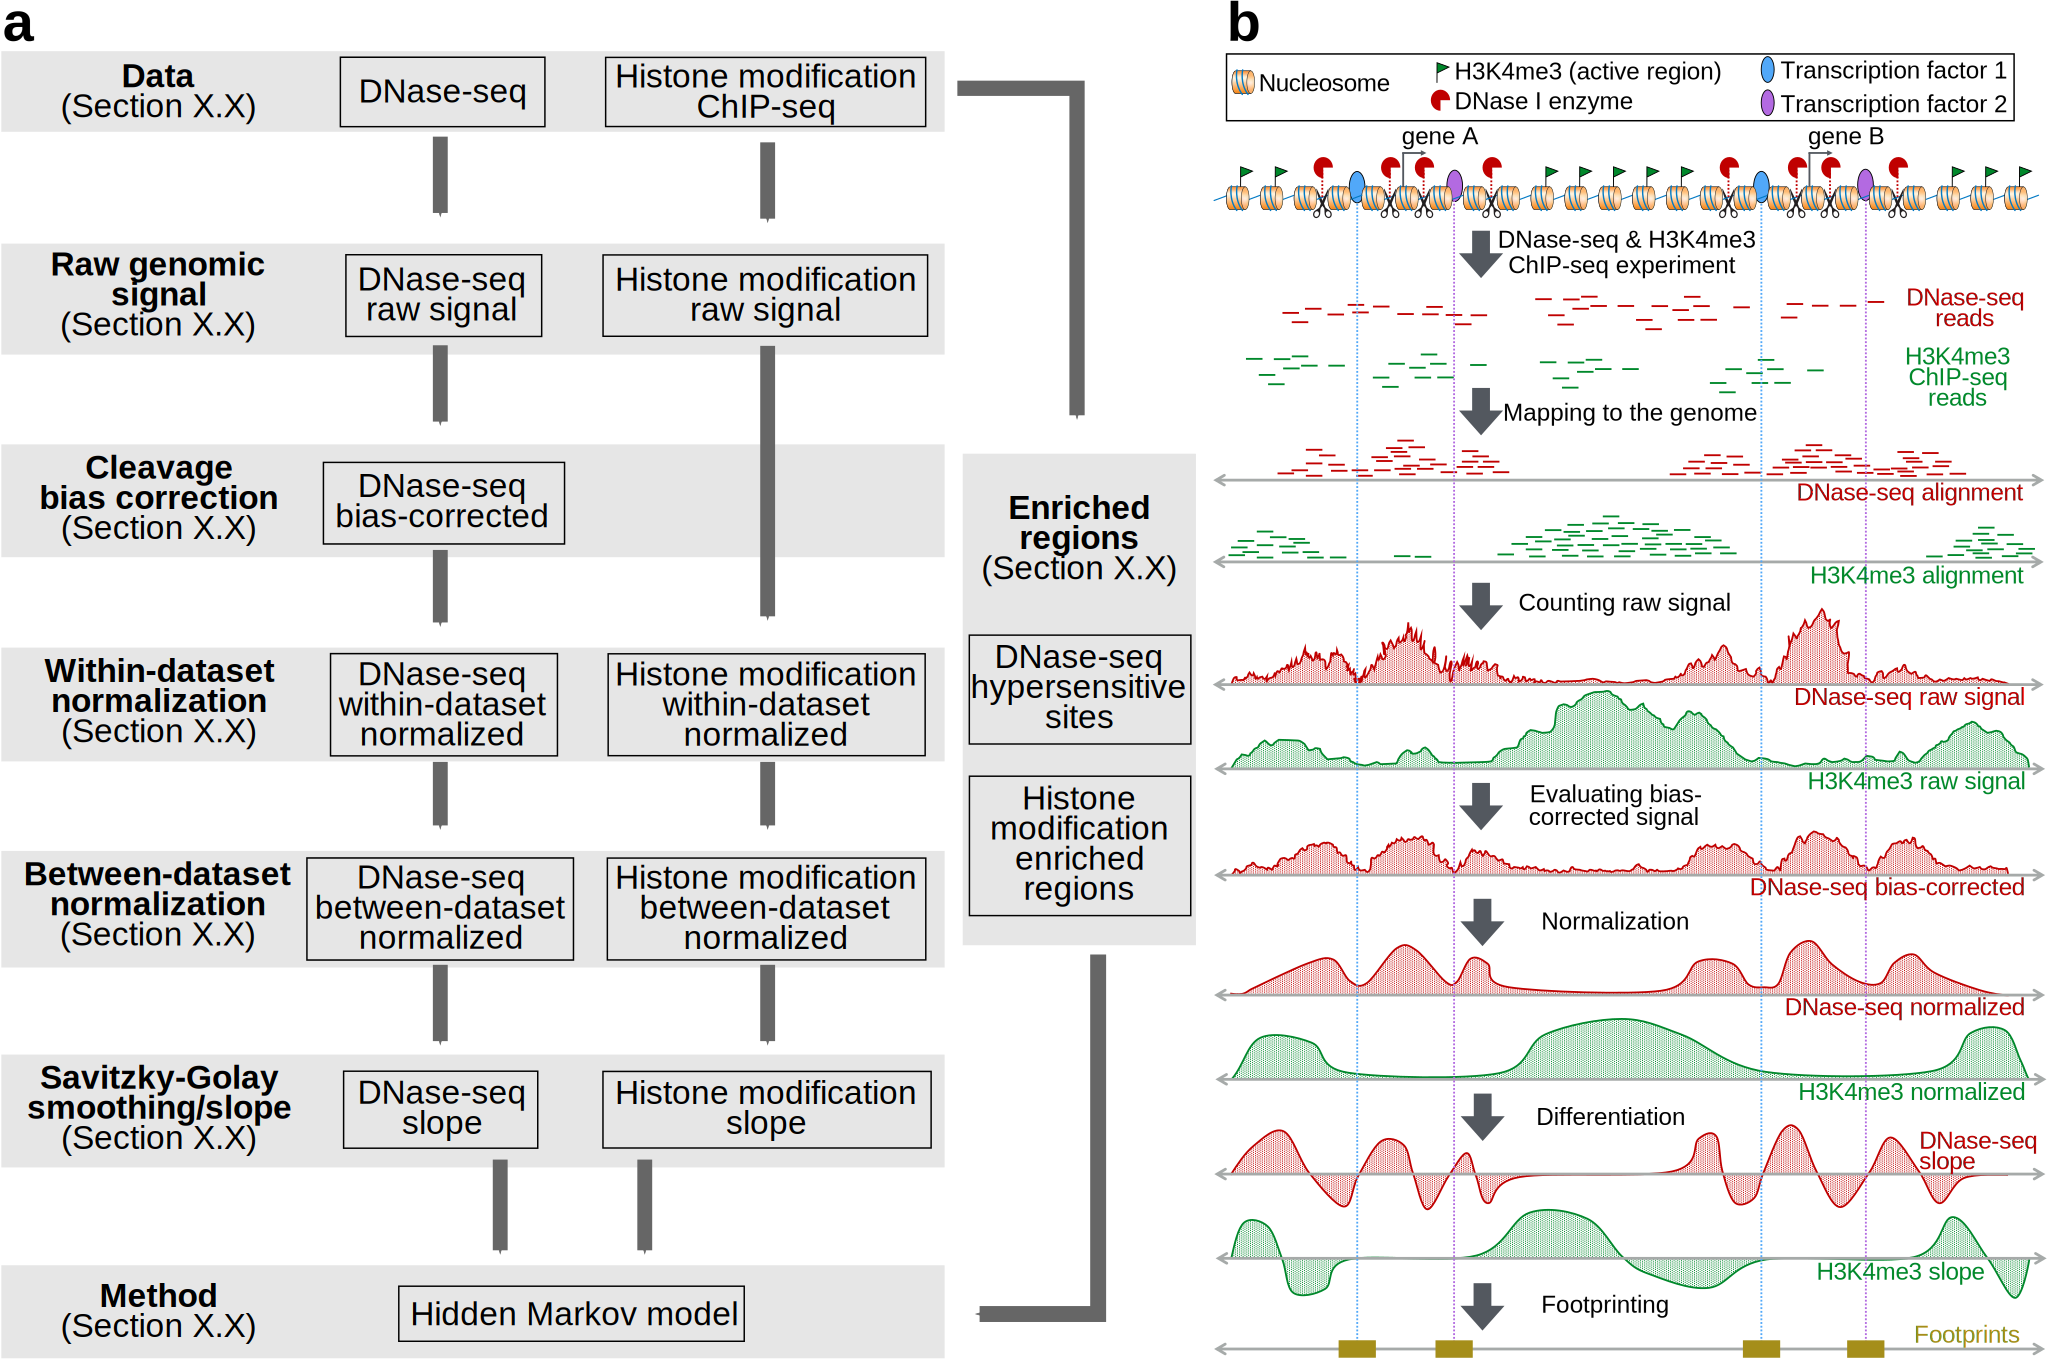
\includegraphics[width=0.99\textwidth]{gusmao_signal_pipeline}
\caption[Input signal processing pipeline]{\textbf{Input signal processing pipeline.} This figure provides a schematic representation of the input signal processing pipeline (left panels) and visual examples of the effects of these processing steps (right panels). The small interval in each genomic signal represents the data scale. \textbf{a} We obtained DNase-seq (always represented in red) and histone modification data (always represented in green) as aligned reads. \textbf{b} A read overlap (raw) signal is generated by counting the number of overlapping aligned tags. Such process is slightly different between DNase-seq and ChIP-seq data.
 \textbf{c} The DNase-seq signal needs to be corrected for sequence cleavage bias. Such correction makes small corretions on the DNase-seq signal as represented by the purple box. \textbf{d} Then, both raw histone modification and cleavage bias-corrected signals are normalized using a within-dataset approach. Such an approach decreases the magnitude differences between the signal peaks within each dataset (see purple dotted line), while preserving the scale of the data. \textbf{e} Afterwards, both signals undergo a between-dataset normalization procedure to allow all data sets to be within the same scale of [0,1]. \textbf{f} The slope of both signals are evaluated using the Savitzky-Golay smoothing filter and differentiation methodology. \textbf{g} The DNase-seq and histone modification normalized and slope signals are the input for our computational footprinting hidden Markov model, which produces footprints. Such step will be expanded in the next section.}
\label{fig:gusmao_signal_pipeline}
\end{figure}

%%%%%%%%%%%%%%%%%%%%%%%%%%%%%%%%%%%%%%%%%%%%%%%%%%%%%%%%%%%%%%%%%%%%%
% Section: Read Overlap Signal
%%%%%%%%%%%%%%%%%%%%%%%%%%%%%%%%%%%%%%%%%%%%%%%%%%%%%%%%%%%%%%%%%%%%%
\subsection{Read Overlap Signal}
\label{sec:read.overlap.signal}

% Genome
Next-generation sequencing (NGS) experiments, such as DNase-seq and ChIP-seq, provides multiple reads, i.e., short DNA sequences that can be aligned into the genome. Here we formally define the genome as a vector
\begin{equation}
  \label{eq:genome}
  \mathbf{g} = \langle {g}_{1}, \cdots, {g}_{n} \rangle,
\end{equation}
where $n$ equals the number of bases (coordinates) in the genome and each ${g}_{i} \in \{\text{A}, \text{C}, \text{G}, \text{T}\}$ represents a nucleotide. As described in Section~\ref{sec:basic.concepts.molecular.biology} the DNA has two strands, which we refer to as the forward and reverse strand. Throughout this thesis consider $\mathbf{g}$ as the forward strand. Strand differentiation will be mentioned only when this issue is important. Moreover, the reverse strand can be inferred from the forward strand since each nucleotide pairs with a specific matching nucleotide.

% Substring
We denote as $\mathbf{g}[u..v]$ a substring of $\mathbf{g}$ from the genomic coordinate $u$ to $v$ for all $u \leq v$, including both within the interval. Therefore, $\mathbf{g}[u..v]$ has total length $u-v+1$. Furthermore, in this thesis we will refer to the term ``genomic region'' to denote an interval from a particular genomic coordinate $u$ to another genomic coordinate $v$. The genomic regions, as the genomic DNA substrings, have both initial ($u$) and final ($v$) positions within the interval and $u \leq v$ for all intervals, which have length $u-v+1$.

% NGS experiments
Furthermore, we can represent the reads obtained from any open chromatin NGS-based experiment, which are aligned into a genome $\mathbf{g}$ as a set of genomic regions (i.e. intervals). Let $ R = \{ {r}_{1}, \cdots, {r}_{m} \}$ be the set of $m$ genomic regions representing the reads from a particular NGS experiment aligned in $\mathbf{g}$. Each ${r}_{i} = [u, v, z]$ represents a triple, where $u$ is the coordinate in $\mathbf{g}$ where the aligned read starts, $v$ is the coordinate in the $\mathbf{g}$ where the aligned read ends and $z \in \{\Plus, \Minus\}$ corresponds to the DNA strand in which the read was aligned to ($\Plus$ represents the forward strand, while $\Minus$ represents the reverse strand).

% Read match/ mismatch
It is important to notice that the actual DNA sequence of the genomic read mapped to positions $u$ to $v$ does not necessarily equal $\mathbf{g}[u..v]$, since we might allow a few mismatches in the string matching alignment algorithm. However, in this project, the DNA sequences of the genomic reads are not important and we will consider only the intervals ${r}_{i}$ in which the reads mapped to the genome $\mathbf{g}$.

% Genomic signal
With such a set $R$ of genomic regions representing the aligned reads we are able to create a genomic signal $\mathbf{x}$, defined as a vector
\begin{equation}
  \label{eq:raw.signal}
  \mathbf{x} = \langle {x}_{1}, \cdots, {x}_{n} \rangle,
\end{equation}
by evaluating the overlap between the aligned reads $R$. However, as previously discussed in Section~\ref{sec:ngs.methods}, only the first base pairs of the DNA fragments obtained from the biological experiments are sequenced by NGS techniques. We are interested in evaluating the overlap of different aligned genomic regions (representing the aligned reads) for different biological experiments (DNase-seq \emph{versus} ChIP-seq). Consequently, we first define a mapping function, which maps a particular read interval to a genomic region based on an extension parameter $\eta$. Such function is written as
\begin{equation}
  \label{eq:raw.signal.extension}
  {f}^{\text{ext}}({r}_{i}, \eta) = {f}^{\text{ext}}([u, v, z], \eta) =
  \begin{cases}
    [u,u+\eta] & \text{if } z = + \\
    [v-\eta,v] & \text{ else.}
  \end{cases}
\end{equation}

% Genomic signal as overlap
With the extension function, we are able to define the overlap signal ($\mathbf{x}$) as
\begin{equation}
  \label{eq:raw.signal.overlap}
  {x}_{i} = \sum_{{r}_{j} \in R} \mathbf{1}\left( i \in {f}^{\text{ext}}({r}_{j}, \eta) \right),
\end{equation}
where ${\mathbf{1}}(\cdot)$ is an indicator function.

% DNase-seq and ChIP-seq extension
The extension parameter $\eta$ used for the DNase-seq is $1$ bp, since we are interested in the regions in which the DNase I enzyme nicked the DNA, i.e. the start of each read. The extension parameter $\eta$ used for ChIP-seq experiments was $200$ bp. Such read size matches the average length of the DNA fragments fetched during the ChIP procedure.

%%%%%%%%%%%%%%%%%%%%%%%%%%%%%%%%%%%%%%%%%%%%%%%%%%%%%%%%%%%%%%%%%%%%%
% Section: DNase-seq Sequence Cleavage Bias
%%%%%%%%%%%%%%%%%%%%%%%%%%%%%%%%%%%%%%%%%%%%%%%%%%%%%%%%%%%%%%%%%%%%%
\subsection{DNase-seq Sequence Cleavage Bias}
\label{sec:dnaseseq.sequence.cleavage.bias}

% Introduction
DNase-seq data was found to be significantly affected by the DNase I sequence cleavage bias~\cite{he2014,meyer2014}. This happens because the DNase I enzyme has an intrinsic preference to bind to (and cleave) certain DNA sequences. In this section we describe our approach to estimate the DNase-seq sequence cleavage bias (Section~\ref{sec:estimation.sequence.cleavage.bias}) and to correct the DNase-seq signal for such bias (Section~\ref{sec:correction.sequence.cleavage.bias}).

%%%%%%%%%%%%%%%%%%%%%%%%%%%%%%%%%%%%%%%%%%%%%%%%%%%%%%%%%%%%%%%%%%%%%
% Section: Estimation of DNase-seq Sequence Cleavage Bias
%%%%%%%%%%%%%%%%%%%%%%%%%%%%%%%%%%%%%%%%%%%%%%%%%%%%%%%%%%%%%%%%%%%%%
\subsubsection{Estimation of DNase-seq Sequence Cleavage Bias}
\label{sec:estimation.sequence.cleavage.bias}

% Introduction
The estimation of DNase-seq experimental bias is performed based on DNA sequence words of length $k$ ($k$-mers). Such estimation is performed in a set of genomic regions of interest $R = \{{r}_{1}, \cdots, {r}_{m}\}$. Our approach consists on measuring, within these genomic regions of interest, the strand-specific: (1) observed DNase I cleavage score for a $k$-mer $\mathbf{w}$, which corresponds to the number of DNase I cleavage sites centered on $\mathbf{w}$; and (2) the background DNase I cleavage score, which is defined by the total number of times $\mathbf{w}$ occurs. Then, the bias estimation is computed as the ratio between the observed and background cleavage scores. Such estimation is performed for all possible $k$-mers within the DNA alphabet $\{\text{A}, \text{C}, \text{G}, \text{T}\}$.

% Strand-specific
The process of estimation and correction of DNase-seq sequence cleavage bias is strand-specific, which means that we will consider the DNA sequences and signal generated separetely for each DNA strand. However, for simplicity of notation, we will not explicitly denote strandedness in the equations.

% Observed cleavage score
For each possible $k$-mer $\mathbf{w}$, which is a string of length $k$ constructed with symbols from the DNA alphabet $\{\text{A}, \text{C}, \text{G}, \text{T}\}$, the strand-specific observed cleavage score ${o}_{\mathbf{w}}$ can be calculated for a set of genomic regions of interest $R = \{r_1, \cdots, r_m\}$ as
\begin{equation}
  \label{eq:obscleav}
  {o}_{\mathbf{w}} = 1 + \sum_{i=1}^{m} \sum_{j \in r_i} {x}_{j} \mathbf{1}\left( \mathbf{g}[j-\frac{k}{2} .. j+\frac{k}{2}] = \mathbf{w}\right).
\end{equation}

% Background cleavage score
Similarly, the background cleavage score ${h}_{\mathbf{w}}$ can be evaluated as
\begin{equation}
  \label{eq:backcleav}
  {h}_{\mathbf{w}} = 1 + \sum_{i=1}^{m} \sum_{j \in r_i} \mathbf{1} \left( \mathbf{g}[j-\frac{k}{2} .. j+\frac{k}{2}] = \mathbf{w}\right).
\end{equation}

% Cleavage bias score
Finally, the estimated cleavage bias ${b}_{i}$ for a genomic position $k+1 \leq i \leq m-k+1$, given that $\mathbf{w}=\mathbf{g}[i-\frac{k}{2}..i+\frac{k}{2}]$, can be calculated as
\begin{equation}
  \label{eq:cleavbias}
  {b}_{i} = \frac{{o}_{\mathbf{w}}}{{h}_{\mathbf{w}}}.
\end{equation}

% Conclusion
The estimated genomic bias signal ${b}_{i}$ represents how many times the $k$-mer sequence $\mathbf{g}[i-\frac{k}{2}..i+\frac{k}{2}+1]$ was cleaved by the DNase I enzyme in comparison to its total occurrence in the set of regions of interest $R$.

%%%%%%%%%%%%%%%%%%%%%%%%%%%%%%%%%%%%%%%%%%%%%%%%%%%%%%%%%%%%%%%%%%%%%
% Section: Correction of DNase-seq Sequence Cleavage Bias
%%%%%%%%%%%%%%%%%%%%%%%%%%%%%%%%%%%%%%%%%%%%%%%%%%%%%%%%%%%%%%%%%%%%%
\subsubsection{Correction of DNase-seq Sequence Cleavage Bias}
\label{sec:correction.sequence.cleavage.bias}

% Introduction
The DNase-seq sequence cleavage bias correction is performed on smoothed versions of both raw DNase-seq ($\mathbf{x}$) and bias score $\mathbf{b}$ signals. The rationale is that we want to avoid dramatic signal changes generated within nucleotide-resolution bias signals.

% Smoothed DNase-seq signal
First, we create a smoothed DNase-seq signal $\hat{\mathbf{x}}$ using a $50$ bp window, which can be written as
\begin{equation}
  \label{eq:smoothed.raw.dnase}
  {\hat{x}}_{i} = \frac{{x}_{j}}{\sum_{j=i-25}^{i+24} {x}_{j}}.
\end{equation}

% Smoothed bias score signal
Then, we create a smoothed bias score signal $\hat{\mathbf{b}}$ using the same $50$ bp window as for the smoothed DNase-seq signal, which can be written as
\begin{equation}
  \label{eq:smoothed.bias.signal}
  {\hat{b}}_{i} = \frac{{b}_{j}}{\sum_{j=i-25}^{i+24} {b}_{j}}.
\end{equation}

% Bias-correction signal
With $\hat{\mathbf{x}}$ and $\hat{\mathbf{b}}$, we are able to calculate a signal of bias-correction factors $\mathbf{c}$ as
\begin{equation}
  \label{eq:bias.corr}
  {c}_{i} = {\hat{x}}_{i} {\hat{b}}_{i}.
\end{equation}

% Pre-processed DNase-seq bias-corrected signal
The pre-processed bias-corrected DNase-seq genomic signal ($\hat{\mathbf{x}}^{\text{bc}}$) is obtained by applying
\begin{equation}
  \label{eq:pre.bias.corr.signal}
  {\hat{x}}_{i}^{\text{bc}} = \log({x}_{i} + 1) - \log({c}_{i} + 1).
\end{equation}

% Global minumum
The pre-processed bias-corrected DNase-seq signal generated by Equation~\ref{eq:pre.bias.corr.signal} may include negative values. Since a few posterior statistical analyses required a signal consisting only of positive values, we have shifted the entire signal by adding the global (genomic) minimum value. The global minimum value $\zeta$ in the pre-processed bias-corrected DNase-seq signal can be evaluated as
\begin{equation}
  \label{eq:pre.dnase.corr.min}
  \zeta = \min_{i = 1, \cdots, n} {\hat{x}}_{i}^{\text{bc}}.
\end{equation}

% DNase-seq bias-corrected signal
Finally, the final DNase-seq bias-corrected signal $\mathbf{x}^{\text{bc}}$ can be evaluated by summing the signals evaluated for each different strand and the global minimum value. Such summation is simply defined as
\begin{equation}
  \label{eq:bias.corr.signal}
  {x}_{i}^{\text{bc}} = {\hat{x}}_{i}^{\text{bc}} + |\zeta| .
\end{equation}
where $|\cdot|$ represents the absolute value of a number.

%%%%%%%%%%%%%%%%%%%%%%%%%%%%%%%%%%%%%%%%%%%%%%%%%%%%%%%%%%%%%%%%%%%%%
% Section: Within-Dataset Normalization
%%%%%%%%%%%%%%%%%%%%%%%%%%%%%%%%%%%%%%%%%%%%%%%%%%%%%%%%%%%%%%%%%%%%%
\subsection{Within-Dataset Normalization}
\label{sec:withindataset.normalization}

% Introduction
The next pre-processing step is applied on both DNase-seq sequence bias-corrected signals and raw histone modification ChIP-seq signals. From this point further, all operations are not strand-specific any longer, since we are dealing only with genomic signals. We will denote both these signals (bias-corrected DNase-seq and raw histone modification ChIP-seq) here as $\mathbf{x}$ for simplicity. This procedure is applied separately on each genomic signal. The within-dataset normalization step aims to reduce the intrinsic variability present within DNase-seq or ChIP-seq data. Such variability arise from the multiple biological and computational protocol steps.

% Genome binning
First, the genome is partitioned into a set of non-overlapping bins ${R} = \{ {r}_{1}, \cdots, {r}_{m} \}$, where each ${r}_{l}$ represents the interval $[((l-1) \cdot \iota )+1, l \cdot \iota]$ for a particular interval-length parameter $\iota$. Furthermore, we also create a genome partition of overlapping bins ${H} = \{ {h}_{1}, \cdots, {h}_{m} \}$, where each ${h}_{l}$ represents the interval ${r}_{l}$ extended by $\iota/2$ on both sides.

% Within-dataset normalization
We are able to create a within-signal normalized signal by dividing the signal by non-zero signal averages~\cite{boyle2011} inside the proposed bins. For a given genomic signal entry $x_i$ at genomic coordinate $i$, such that $i \in {r}_{l}$, we apply
\begin{equation}
  \label{eq:signal.within.norm}
  {x}^{\text{norm1}}_{i} = \frac{{x}_{i}}{ 
                     \sum\limits_{j \in {h}_{l}} {x}_{j} \mathbf{1}({x}_{j} > 0)  \;\; \Big/  
                     \sum\limits_{j \in {h}_{l}} \mathbf{1}({x}_{j} > 0)
                     }.
\end{equation}

%%%%%%%%%%%%%%%%%%%%%%%%%%%%%%%%%%%%%%%%%%%%%%%%%%%%%%%%%%%%%%%%%%%%%
% Section: Between-Dataset Normalization
%%%%%%%%%%%%%%%%%%%%%%%%%%%%%%%%%%%%%%%%%%%%%%%%%%%%%%%%%%%%%%%%%%%%%
\subsection{Between-Dataset Normalization}
\label{sec:betweendataset.normalization}

% Introduction
After the within-dataset normalization, we perform a between-dataset normalization procedure to force values inside the interval $ [0,1] $ by fitting the within-dataset normalized signals into a logistic function. Differently from the within-dataset normalization, which must be performed in a local manner, the between-dataset normalization can be performed using either a local or global approach. Here we describe both procedures.

% Between-dataset normalization - local approach
\subsubsection{Local Appoach}

% Between-dataset normalization - local approach
Let ${R} = \{ {r}_{1}, \cdots, {r}_{m} \}$ and ${H} = \{ {h}_{1}, \cdots, {h}_{m} \}$ be non-overlapping and overlapping genomic partitions, respectivelly, as described in Section~\ref{sec:withindataset.normalization}. For a given genomic signal entry $x_i$ at genomic coordinate $i$, such that $i \in {r}_{l}$, we apply
\begin{equation}
  \label{eq:signal.between.norm.local}
  {x}^{\text{norm2}}_{i} = \frac{1}{1+e^{{-({x}^{\text{norm1}}_{i}-{\varsigma}^{t}_{{h}_{l}})}/{\sigma}_{{h}_{l}}}},
\end{equation}
where ${\varsigma}^{t}_{{h}_{l}}$ is the $t^{\text{th}}$ percentile of the signal data points within the interval ${h}_{l}$ and $\sigma_{{h}_{l}}$ is the standard deviation of the signal data points within the interval ${h}_{l}$, given by
\begin{equation}
  \label{eq:signal.between.var.local}
  \sigma_{{h}_{l}} = \sqrt{ \frac{\sum_{j \in {h}_{l}} \left({x}^{\text{norm1}}_{j} - \mu_{{h}_{l}}\right)^2}{2\iota} },
\end{equation}
where $\mu_{{h}_{l}}$ is the mean of the signal data points within the interval ${h}_{l}$, given by
\begin{equation}
  \label{eq:signal.between.mean.local}
  \mu_{{h}_{l}} = \sum_{j \in {h}_{l}} \frac{{x}^{\text{norm1}}_{j}}{2\iota}.
\end{equation}

% Between-dataset normalization - global approach
\subsubsection{Global Appoach}

% Between-dataset normalization - global approach
The global approach for the between-dataset normalization procedure follows the same idea of the local approach. However, the signal's mean, standard deviation and percentile are evaluated globally. For a given genomic signal entry $x_i$ at genomic coordinate $i$, the global between-dataset normalization is written as
\begin{equation}
  \label{eq:signal.between.norm.global}
  {x}^{\text{norm2}}_{i} = \frac{1}{1+e^{{-({x}^{\text{norm1}}_{i}-{\varsigma}^{t})}/{\sigma}}},
\end{equation}
where ${\varsigma}^{t}$ is the $t^{\text{th}}$ percentile of $\mathbf{x}^{\text{norm2}}$ and $\sigma$ is the standard deviation of $\mathbf{x}^{\text{norm2}}$, given by
\begin{equation}
  \label{eq:signal.between.var.global}
  \sigma = \sqrt{ \frac{\sum_{j=1}^{n} \left({x}^{\text{norm1}}_{j} - \mu \right)^2}{ n }},
\end{equation}
where $\mu$ is the mean of $\mathbf{x}^{\text{norm2}}$, given by
\begin{equation}
  \label{eq:signal.between.mean.global}
  \mu = \sum_{j=1}^{n} \frac{{x}^{\text{norm1}}_{j}}{n}.
\end{equation}

% Normalized signal
After the application of the within-dataset and between-dataset normalization procedures (for both DNase-seq and histone modification ChIP-seq), we consider the output as our ``normalized'' signal. Such normalized signals will represent some of the input signals to our method.

%%%%%%%%%%%%%%%%%%%%%%%%%%%%%%%%%%%%%%%%%%%%%%%%%%%%%%%%%%%%%%%%%%%%%
% Section: Savitzky-Golay Smoothing and Slope
%%%%%%%%%%%%%%%%%%%%%%%%%%%%%%%%%%%%%%%%%%%%%%%%%%%%%%%%%%%%%%%%%%%%%
\subsection{Savitzky-Golay Smoothing and Slope}
\label{sec:savitzkygolay.smoothing.slope}

% Introduction
As it will be clearer when we describe our computational footprinting framework in Section~\ref{sec:computational.footprinting.hmm}, we need an additional signal, which indicates upward and downward trends in the normalized genomic signals. We will use the slope of the normalized signal to assess such information. In order to estimate the slope of the genomic signals we apply a Savitzky-Golay smoothing filter followed by differentiation~\cite{madden1978,luo2005}.

% Savitzky-Golay smoothing and differentiation
The Savitzky-Golay smoothing filter and differentiation method consists of fitting the data into a polynomial, performing a convolution (based on a specific window length $\tau$) with a vector containing Savitzky-Golay coefficients~\cite{madden1978}.

% Savitzky-Golay convolution
Let an odd-number $\tau$ be a specific window length in which the smoothing is going to be performed. The Savitzky-Golay convolution can be expressed as
\begin{equation}
  \label{eq:slope}
  {x}^{\text{slope}}_{i} = \sum\limits_{j=-\frac{\tau-1}{2}}^{\frac{\tau-1}{2}} {c}_{j+\frac{\tau-1}{2}} {x}^{\text{norm2}}_{i+j},
\end{equation}
where $\mathbf{c}$ is the vector of Savitzky-Golay coefficients.

% Savitzky-Golay coefficients
The derivation of the Savitzky-Golay coefficients can be performed using an analytical solution that enables the smoothing and differentiation within the same convolution depicted in Equation~\ref{eq:slope}. First, a polynomial will be fitted by linear least squares to a set of $\tau$ adjacent data points. These are the same data points within the window of the convolution represented in Equation~\ref{eq:slope}. Then, let $\mathbf{z}$ be a variable which represents the index of the equally-spaced convolution, i.e. $\mathbf{z} = \{ {z}_{1}, {z}_{2}, \cdots, {z}_{\tau} \} = \{ -\frac{\tau-1}{2}, \cdots, 0, \cdots, \frac{\tau-1}{2}\}$. The fitted polynomial of degree $\tau$ can be described as
\begin{equation}
  \label{eq:sg.polynomial}
  Y = {c}_{0} + {c}_{1}{z} + {c}_{2}{z}^{2} + {c}_{\tau}{z}^{\tau}.
\end{equation}

% Jacobian matrix
The coefficients $c_i$ are obtained by solving the linear square's normal equations
\begin{equation}
  \label{eq:savitzky.golay.coeff}
  \mathbf{c} = {\left( \mathbf{J}^{\intercal} \mathbf{J} \right)}^{-1} \mathbf{J}^{\intercal} \mathbf{\hat{x}},
\end{equation}
where $\mathbf{\hat{x}} $ is the vector of signals within the current convolution window of length $\tau$ (see Equation~\ref{eq:slope}), and the  $i^{\text{th}}$ row of the Jacobian matrix $\mathbf{J}$, denoted as
\begin{equation}
  \label{eq:savitzky.golay.jacob}
  \frac{\partial \mathbf{\hat{x}} }{\partial \mathbf{c}},
\end{equation}
has values $ \langle 1, {z}_{i}, {z}_{i}^{2}, \cdots, {z}_{i}^{\tau} \rangle$.

% Full derivation
For the full linear squares derivation of the Savitzky-Golay coefficients and more details on the effects of such smoothing filter, please refer to Luo et al.~\cite{luo2005}.

%%%%%%%%%%%%%%%%%%%%%%%%%%%%%%%%%%%%%%%%%%%%%%%%%%%%%%%%%%%%%%%%%%%%%
% Section: Computational Footprinting with Hidden Markov Models
%%%%%%%%%%%%%%%%%%%%%%%%%%%%%%%%%%%%%%%%%%%%%%%%%%%%%%%%%%%%%%%%%%%%%
\section{Computational Footprinting with Hidden Markov Models}
\label{sec:computational.footprinting.hmm}

% Introductions
In order to detect footprints in genomic signals of the DNase-seq and histone modification experiments we need a technique which is able to segment the genome and cope with input multidimensionality. The grammar of active transcription factor binding sites shows a clear temporal pattern in which active transcription factors bind the genome. However, the length of each of these pattern's segment, i.e. length of the background regions (with no detectable signals), the length of histone or DNase peaks and the duration of the footprints are intrinsically diverse. Furthermore, segmented regions might present a similar level of the signals. For instance, both the background genomic regions and footprint genomic regions, which should definetly be separated by the computational footprinting segmentation method, have the same signal landscape, i.e. low absolute (close to zero) signals of both DNase-seq and histone modification ChIP-seq signals. The difference between these regions is that the footprint happen within two peaks of DNase-seq signals, which happen within two peaks of active histone modification signals. Given these remarks, the best method of choice for such a segmentation task are hidden Markov models (HMMs). Hidden Markov model (HMM) is a computational technique based on the Bayes probability theory and Markov stochastic processes. Such computational model is defined thoroughly in Section~\ref{sec:multivariate.continuous.hmm}.

% Computational footprinting with HMMs
After defining the HMMs, we proceed to discuss how this probabilistic model can be used to segment the genome in the context of the identification of active transcription factor binding sites. The Figure~\ref{fig:gusmao_method_pipeline} shows a schematic pipeline of our computational footprinting framework using HMMs. First, we define a number of different model topologies based on the grammar of active transcription factor binding sites and on remarks made by recent studies on the heterogeneity of such grammar (Section~\ref{sec:hmm.topology}). The different HMM topologies takes different signals, which can be normalized and/or slope versions of the DNase-seq (Figure~\ref{fig:gusmao_method_pipeline}a) and histone modification ChIP-seq (Figure~\ref{fig:gusmao_method_pipeline}b) signals. All HMM topologies used in this thesis can be seen in Figure~\ref{fig:gusmao_method_pipeline}c--g. Next, we define how the model can be trained in a supervised manner, using annotation of known transcription factor binding sites and a maximum-likelihood probability approach (Section~\ref{sec:hmm.training}; Figure~\ref{fig:gusmao_method_pipeline}h). The DNase-seq and histone modification ChIP-seq data can then be used as input for the trained HMMs to make predictions of active transcription factor binding sites (Section~\ref{sec:hmm.decoding}). To acomplish such a task, we tried two different decoding methods -- the Viterbi algorithm and the calculation of the HMM's posterior probability (Figure~\ref{fig:gusmao_method_pipeline}i). Finally, we present the post-processing steps applied on the predicted active transcription factor binding sites, i.e. footprints (Section~\ref{sec:footprint.postprocessing}).

% Figure - Computational footprinting framework
\begin{figure}[h!]
\centering
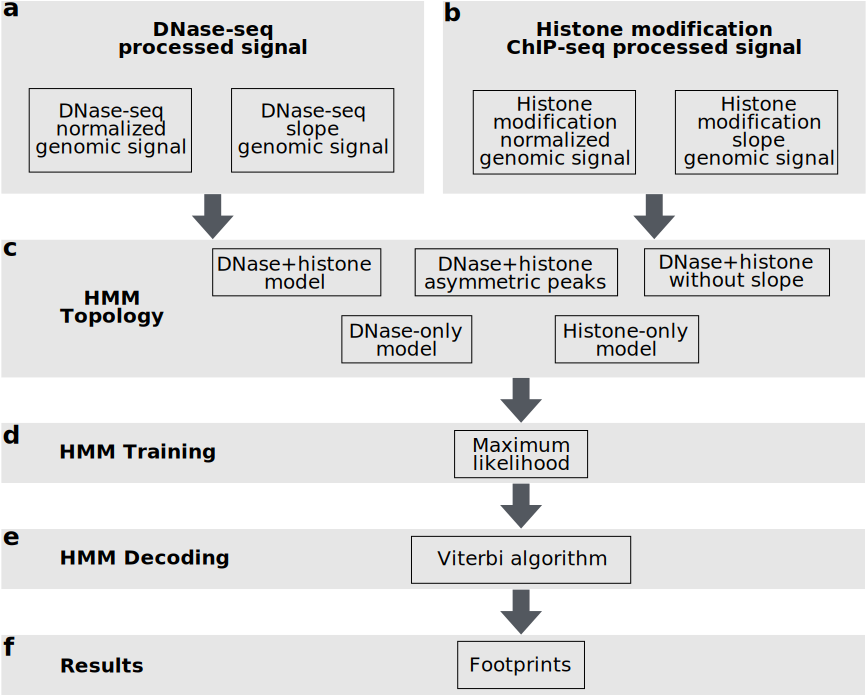
\includegraphics[width=0.97\textwidth]{gusmao_method_pipeline}
\caption[Computational footprinting framework]{\textbf{Computational footprinting framework.} Graphical representation of the computational footprinting method pipeline. (\textbf{a},\textbf{b}) Different HMM models take normalized and/or slope signals of DNase-seq and/or histone modification ChIP-seq. (\textbf{c}--\textbf{g}) Different HMM topologies were used. (\textbf{h}) All HMM models are trained using the supervised maximum likelihood method. (\textbf{i}) We used two decoding methods to apply the HMM in the genomic signal and predict footprints: (1) the Viterbi algorithm and (2) the calculation of the posterior probability. (\textbf{j}) The final footprints are available after a few post-processing steps.}
\label{fig:gusmao_method_pipeline}
\end{figure}

%%%%%%%%%%%%%%%%%%%%%%%%%%%%%%%%%%%%%%%%%%%%%%%%%%%%%%%%%%%%%%%%%%%%%
% Section: Multivariate Continuous HMM
%%%%%%%%%%%%%%%%%%%%%%%%%%%%%%%%%%%%%%%%%%%%%%%%%%%%%%%%%%%%%%%%%%%%%
\subsection{Multivariate Continuous HMM}
\label{sec:multivariate.continuous.hmm}

% Introduction
Markov chains are probabilistic models composed by a collection of states and transitions between these states, which correspond to the probability of changing between states. The hidden Markov models follow the same baseline idea, however they also contain within their model an unknown sequence of states associated to each input symbol. In this section we formalize the concept of hidden Markov models.

% Parameters
Let $\mathbf{X}^{d \times n}$ be a matrix of $d$ observed multivariate continuous genomic signals, each of which has length $n$. For a given multivariate observation $\langle \mathbf{{x}_{\cdot 1}}, \cdots, \mathbf{{x}_{\cdot t}}, \cdots, \mathbf{{x}_{\cdot n}} \rangle$ from $\mathbf{X}$, we have a corresponding hidden sequence path $\mathbf{q} = \langle q_1, \cdots, q_t, \cdots, q_n \rangle$, where $ q_t \in \Psi = \{1, \cdots, \psi\} $ represents the state emitting the vector $ {\mathbf{x}}_{\cdot t} $ at the $t^{\text{th}}$ genomic position. Then, we define a multivariate continuous HMM as the set of parameters
\begin{equation}
  \label{eq:hmm.theta}
  \Theta= \{\mathbf{A}, \mathbf{E}, \mathbf{s}\}.
\end{equation}

% Transitions
$\mathbf{A}$ represents the matrix which contains the mass probabilities of transitioning between the states of the HMM. We formalize this as
\begin{equation}
  \label{eq:hmm.a}
  \mathbf{A} = {\{a_{uv}\}}^{\psi \times \psi},
\end{equation}
where $\psi$ is the number of states within the HMM topology and $a_{uv}$ represents the mass probability of transition from state $u$ to $v$, which is
\begin{equation}
  \label{eq:hmm.transition}
  a_{uv} = P(q_t = v | q_{t-1} = u).
\end{equation}

% Emission
$\mathbf{E}$ represents the set of emission probabilities. We define $\mathbf{E}$ as a vector of probability density functions
\begin{equation}
  \label{eq:hmm.e}
  \mathbf{E} = \langle e_1(\mathbf{x}), \cdots, e_{\psi}(\mathbf{x}) \rangle,
\end{equation}
where each state $u$ has a probability $e_u(\mathbf{x})$ of emitting the vector symbol $ \mathbf{x} $. Such probability density function is represented by
\begin{equation}
  \label{eq:hmm.emission}
  e_u(\mathbf{x}) = p( \mathbf{{x}_{\cdot t}} | q_t = u).
\end{equation}
The probability density function used for the emission probabilities correspond to a multivariate normal density function with full covariance matrix. This is described as
\begin{equation}
  \label{eq:hmm.emission.gaussian}
  \begin{array}{lcl}
    p(\mathbf{{x}_{\cdot t}} | q_t = u) & = & 
    p(\mathbf{x_{\cdot t}}|{{\boldsymbol\mu}^{\mathbf{u}}},{{\boldsymbol\Sigma}^{\mathbf{u}}})\\[0.4em] & = &
    \frac{1}{ \sqrt{(2\pi)^{D} {| {{\boldsymbol\Sigma}^{\mathbf{u}}} |}}}
    e^{-\frac{1}{2} (\mathbf{x_{\cdot t}}-{{\boldsymbol\mu}^{\mathbf{u}}})^T ({{\boldsymbol\Sigma}^{\mathbf{u}}})^{-1} (\mathbf{x_{\cdot t}}-{{\boldsymbol\mu}^{\mathbf{u}}})}, \\
  \end{array}
\end{equation}
where ${{\boldsymbol\mu}^{\mathbf{u}}}$ and ${{\boldsymbol\Sigma}^{\mathbf{u}}}$ are, respectively, the $d$-dimensional mean vector and full covariance matrix of the emission probability density function at state $u$.

% Initial state probabilities
$\mathbf{s}$ represents the initial set of transition probabilities. Such parameter is required to ``start'' the model at a given set of states. The initial state transition probabilities are represented as a vector of mass probabilities
\begin{equation}
  \label{eq:hmm.initial}
  \mathbf{s} = \langle s_{1}, \cdots, s_{\psi} \rangle.
\end{equation}

% Independence assumptions
There are two independence assumptions which need to be made in order to be able to work with the aforementioned proposed HMM. The first assumption is that the probability to reach state $t$ depends only on the previous state $t-1$
\begin{equation}
  \label{eq:hmm.indep.1}
  p(q_t | q_1, \cdots, q_{t-1}) = p(q_t | q_{t-1}),
\end{equation}
and the second assumption dictates that the density function of emitting an input vector $\mathbf{{x}_{\cdot t}}$ observed at state $t$, depends only at this current state
\begin{equation}
  \label{eq:hmm.indep.2}
  p(\mathbf{{x}_{\cdot t}} | q_1, \cdots, q_t) = p(\mathbf{{x}_{\cdot t}} | q_t).
\end{equation}

% HMM problems - intuition 1
Given the formalism previously defined, there are three general problems on which we can address directly through computationally efficient implementations of HMMs:

\begin{center}
  \begin{tabular}{lp{.8\linewidth}}
    {\bf Problem 1} & Estimate the HMM parameters $ \Theta $ in order to maximize $p(\mathbf{X} | \Theta)$. \\[0.2cm]
    {\bf Problem 2} & Given an observed multivariate input $ \mathbf{X} $ and an HMM model represented by the parameters $ \Theta $, find the sequence of hidden states $ \mathbf{q} $ which best explains the input given the HMM model, i.e. that maximizes $ p\left( \mathbf{X}, \mathbf{q} | \Theta \right) $ . \\[0.2cm]
    {\bf Problem 3} & Given an observed multivariate input $ \mathbf{X} $ and an HMM model represented by the parameters $ \Theta $, compute the probability of the input sequence given the HMM model $p(\mathbf{X} | \Theta)$. \\[0.2cm]
  \end{tabular}
\end{center}

% HMM problems - intuition 2
The first problem regards the HMM parameter estimation, i.e. model training. This problem will be addressed in Section~\ref{sec:hmm.training}. The second and third problems represent our genomic segmentation methodology using the HMM states in order to predict active binding sites. These problems will be explored in Section~\ref{sec:hmm.decoding}. For a more thorough discussion, including proof of theorems, we refer to a number of publications~\cite{rabiner1989,durbin1998,mitchell1997,bishop2006,duda2000}.

%%%%%%%%%%%%%%%%%%%%%%%%%%%%%%%%%%%%%%%%%%%%%%%%%%%%%%%%%%%%%%%%%%%%%
% Section: HMM Topology
%%%%%%%%%%%%%%%%%%%%%%%%%%%%%%%%%%%%%%%%%%%%%%%%%%%%%%%%%%%%%%%%%%%%%
\subsection{HMM Topology}
\label{sec:hmm.topology}

% Introduction
We refer to HMM topology as the number of states $\psi$ and the pre-defined possible transitions between these states ($a_{uv} > 0$). The mathematical modelling of a problem with HMMs require the knowledge of the problem in order to be able to create a meaningful HMM topology. We implemented a number of different HMM topologies, depicted in Figure~\ref{fig:gusmao_method_pipeline}c--g. It is important to mention that all HMM states from all topologies have transitions to itself, which were omitted for simplicity. In this section we will define these topologies and discuss the rationale behind each topology choice. To enhance clarity, the HMM states will also be represented with labels using the {\tt UPPERCASE COURRIER} font.

% DNase + Histone HMM -- Model 1
\subsubsection{DNase + Histone HMM -- Model 1}

% Introduction
The DNase + Histone HMM Model 1 (M1; Figure~\ref{fig:gusmao_method_pipeline}c) represents our main topology. It combines both DNase-seq and histone modification ChIP-seq in an HMM structure devised to recognize the grammar of active TFBS described in Section~\ref{sec:grammar.tfbs}.

% Signal
In this topology, the input matrix $\mathbf{X}$ can be represented as a vector of input signal vectors
\begin{equation}
  \label{eq:signal.m1}
  \mathbf{X} = \langle \quad \mathbf{x}^{\text{norm2}}_{\text{dnase}} \quad \mathbf{x}^{\text{slope}}_{\text{dnase}} \quad \mathbf{x}^{\text{norm2}}_{\text{histone}} \quad \mathbf{x}^{\text{slope}}_{\text{histone}} \quad \rangle .
\end{equation}

% Topology
The first state ({\tt BACK}) corresponds to the ``background'' regions with low concentration of DNase-seq and histone modification ChIP-seq signals. The histone level states represent a peak in the histone modification ChIP-seq signal, recognizing an increase in the histone modification ChIP-seq signal based on high positive $x^{\text{slope}}_{\text{histone}\ \cdot}$ values ({\tt UP}), summit regions with $x^{\text{slope}}_{\text{histone}\ \cdot}$ values close to zero with high $x^{\text{norm2}}_{\text{histone}\ \cdot}$ values ({\tt TOP}) and a decrease based on negative values of the $x^{\text{slope}}_{\text{histone}\ \cdot}$ signal ({\tt DOWN}). From the histone level {\tt DOWN} state, the model can either return to {\tt BACK} (isolated histone modification peaks without further DHSs) or continue to the DNase level {\tt UP} state. The DNase level states are equivalent to the histone level states, with the exception that the $x^{\text{norm2}}_{\text{dnase}\ \cdot}$ and $x^{\text{slope}}_{\text{dnase}\ \cdot}$ signals are being recognized instead. From the DNase level {\tt DOWN} state, the model decides between returning to a region of higher histone modification ChIP-seq signals (histone level {\tt UP} state) and visiting the {\tt FOOTPRINT} state, which represents the dip between two peaks of intense DNase I cleavage. The regions of the genome where the HMM has recognized as {\tt FOOTPRINT} are the ones reported by our method as likely TFBSs.

% Figure intro
The Figure~\ref{fig:gusmao_hmm_footprinting} depicts such HMM topology and an example of a genomic region annotated by such HMM.

% Figure - Example of HMM topology and genomic segmentation
\begin{figure}[h!]
\centering
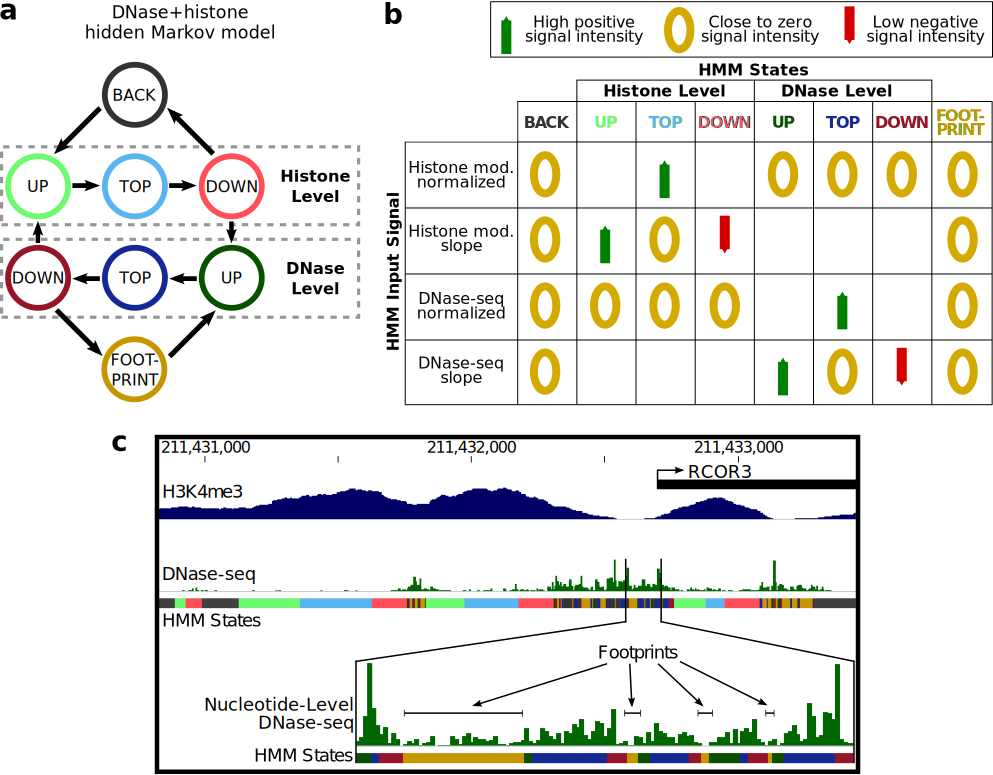
\includegraphics[width=0.99\textwidth]{gusmao_hmm_footprinting}
\caption[Example of HMM topology and genomic segmentation]{\textbf{Example of HMM topology and genomic segmentation.} (\textbf{a}) DNase-seq and H3K4me3 (ChIP-seq) profiles around the promoter region of RCOR3 -- REST corepressor 3 on K562 cell type. The DNase-seq signal indicates three clear DHSs (HS1, HS2 and HS3), each of which fits dip regions within the H3K4me3 signal. Moreover, these regions consist of several putative footprints of varied sizes. (\textbf{b}) Eight state HMM proposed. The first state models background signal ({\tt BACK}). From the background state, the only possible transition is to the histone level states, which will model the increase ({\tt UP}), high levels ({\tt TOP}) and decrease ({\tt DOWN}) of histone modifications. After visiting histone level states, the HMM allows transitions to the DNase level states, which again model the increase, high levels and decrease in the DHS signal. Only then, the {\tt FOOTPRINT} state can be visited. After a footprint visit, the HMM has to go again to the DNase and histone level states, emphasizing the peak-dip-peak pattern.}
\label{fig:gusmao_hmm_footprinting}
\end{figure}

% DNase + Histone HMM -- Model 2
\subsubsection{DNase + Histone HMM -- Model 2}

% Introduction
The DNase + Histone HMM Model 2 (M2; Figure~\ref{fig:gusmao_method_pipeline}d) is an extension of the DNase + Histone MMM Model 1 to account for the histone modification signal asymmetry, i.e. that some DHSs have very small signals of active histone modifications on its downstream or upstream regions~\cite{kundaje2012}. For such, two additional transitions were added (shown in red in Figure~\ref{fig:gusmao_method_pipeline}d) in order to allow the DNase level states to be visited when there are no histone modification peaks before or after DNase-seq peaks.

% Signal
In this topology, the input matrix $\mathbf{X}$ is the same as depicted for the DNase + Histone MMM Model 1 in Equation~\ref{eq:signal.m1}.

% DNase + Histone HMM -- Model 3
\subsubsection{DNase + Histone HMM -- Model 3}

% Introduction
The DNase + Histone HMM Model 3 (M3; Figure~\ref{fig:gusmao_method_pipeline}f) is a simplification of the DNase + Histone MMM Model 1, which performs the predictions of footprints without the slope signal. In DNase + Histone HMM Model 3, the {\tt UP}, {\tt TOP} and {\tt DOWN} states from DNase + Histone MMM Model 1 are compressed into one state -- {\tt HIGH} -- which recognizes high levels of DNase-seq cleavage activity (DNase level state) or high levels of histone modifications (histone level state).

% Signal
In this topology, the HMM needs only the normalized signal and becomes bivariate (DNase-seq and histone modifications normalized signals). The input matrix $\mathbf{X}$ can be represented as a vector of input signal vectors
\begin{equation}
  \label{eq:signal.m3}
  \mathbf{X} = \langle \quad \mathbf{x}^{\text{norm2}}_{\text{dnase}} \quad \mathbf{x}^{\text{norm2}}_{\text{histone}} \quad \rangle .
\end{equation}

% DNase-only HMM
\subsubsection{DNase-only HMM}

% Introduction
The DNase-only HMM (Figure~\ref{fig:gusmao_method_pipeline}e) represents an alternative model to the DNase + Histone MMM Model 1. Such model uses only DNase-seq signal and the following modifications were performed in comparison to the DNase + Histone MMM Model 1. The histone level states were removed and additional transitions were added: (1) from the DNase level {\tt DOWN} state to the {\tt BACK} state and (2) from the {\tt BACK} state to the DNase level level {\tt UP} state.

% Signal
In this topology, the input matrix $\mathbf{X}$ can be represented as a vector of DNase-seq input signal vectors
\begin{equation}
  \label{eq:signal.m4}
  \mathbf{X} = \langle \quad \mathbf{x}^{\text{norm2}}_{\text{dnase}} \quad \mathbf{x}^{\text{slope}}_{\text{dnase}} \quad \rangle .
\end{equation}

% Histone-only HMM
\subsubsection{Histone-only HMM}

% Introduction
The Histone-only HMM (Figure~\ref{fig:gusmao_method_pipeline}g) represents an alternative model to the DNase + Histone MMM Model 1. Such model uses only histone modification ChIP-seq signal. The changes in comparison to the DNase + Histone MMM Model 1 are exactely the same as for the DNase-only model; however, instead of removing the histone level states, the DNase level states are removed and additional transitions are created: (1) from the histone level {\tt DOWN} state to the {\tt FOOTPRINT} state and (2) from the {\tt FOOTPRINT} state to the histone level level {\tt UP} state.

% Signal
In this topology, the input matrix $\mathbf{X}$ can be represented as a vector of histone modification ChIP-seq input signal vectors
\begin{equation}
  \label{eq:signal.m5}
  \mathbf{X} = \langle \quad \mathbf{x}^{\text{norm2}}_{\text{histone}} \quad \mathbf{x}^{\text{slope}}_{\text{histone}} \quad \rangle .
\end{equation}

%%%%%%%%%%%%%%%%%%%%%%%%%%%%%%%%%%%%%%%%%%%%%%%%%%%%%%%%%%%%%%%%%%%%%
% Section: HMM Training
%%%%%%%%%%%%%%%%%%%%%%%%%%%%%%%%%%%%%%%%%%%%%%%%%%%%%%%%%%%%%%%%%%%%%
\subsection{HMM Training}
\label{sec:hmm.training}

% Training A
We estimate the HMM parameters in a supervised manner, using the maximum likelihood method. For a given annotation sequence of the HMM states $\mathbf{q} = \langle q_1, \cdots, q_t, \cdots, q_n \rangle$ and sample data $\mathbf{X}$, the transition mass probabilities can be estimated as
\begin{equation}
  \label{eq:hmm.train.a.1}
  a_{uv} = \frac{ \hat{a}_{uv}}{ \sum_{w=1}^{\psi} \hat{a}_{uw}},
\end{equation}
where $ \hat{a}_{uv} $ represents the number of transitions from state~$u$ to state~$v$ observed in the annotated training data, formally defined as
\begin{equation}
  \label{eq:hmm.train.a.2}
  \hat{a}_{uv} = \sum_{i=1}^{n-1} \mathbf{1} (q_i=u, q_{i+1}=v).
\end{equation}

% Training E
The emission probability density functions (gaussian distributions) are estimated as
\begin{equation}
  \label{eq:hmm.train.e.1}
  \mu^{u}_{i} = \frac{ \sum_{j=1}^{n} {x}_{ij} {\mathbf{1}}(q_j=u) }{ \sum_{j=1}^{n} {\mathbf{1}} (q_j=u) },
\end{equation}
where $ \mu^{u}_{i} $ is the gaussian's mean at state $u$ for the signal $i$ and
\begin{equation}
  \label{eq:hmm.train.e.2}
  {\sigma}^{u}_{ik} = \frac{\sum_{j=1}^{n} ({x}_{ij} - \mu^{u}_{i})^T({x}_{kj} - \mu^{u}_{k}) {\mathbf{1}} (q_j=u)}
  {\sum_{j=1}^{n} {\mathbf{1}} (q_j=u) - 1}.
\end{equation}
where $ \sigma^{u}_{ik} $ is the gaussian's variance at state $u$ between signals $i$ and $k$.

% Training s
As we expect the HMM to always start at the {\tt BACK} state (the first HMM state), the initial transition vector $\mathbf{s}$ was manually set with the following probabilities
\begin{equation}
  \label{eq:hmm.train.s}
  \begin{array}{lcl}
    s_1 = 1 \\
    s_t = 0 \quad \forall \quad t \neq 1 \\
  \end{array}.
\end{equation}

%%%%%%%%%%%%%%%%%%%%%%%%%%%%%%%%%%%%%%%%%%%%%%%%%%%%%%%%%%%%%%%%%%%%%
% Section: HMM Decoding
%%%%%%%%%%%%%%%%%%%%%%%%%%%%%%%%%%%%%%%%%%%%%%%%%%%%%%%%%%%%%%%%%%%%%
\subsection{HMM Decoding}
\label{sec:hmm.decoding}

% Introduction
Given HMMs with topologies described in Section~\ref{sec:hmm.topology} and parameters estimated as described in Section~\ref{sec:hmm.training} we are able to perform the prediction of active transcription factor binding sites. We can predict active TFBSs using two approaches which are computationally feasible. The first -- termed Viterbi algorithm -- address the {\bf Problem 2} defined in Section~\ref{sec:multivariate.continuous.hmm}. Briefly, it computes the sequence of hidden states $ \mathbf{q} $ that maximizes $ p\left( \mathbf{X}, \mathbf{q} | \Theta \right) $. Then, given the computated sequence of hidden states we are able to identify the ones which corresponds to the {\tt FOOTPRINT} state and regard these regions as the active transcription factor binding sites. This algorithm will be described in Section~\ref{sec:viterbi.algorithm}. Furthermore, we can address the {\bf Problem 3} defined in Section~\ref{sec:multivariate.continuous.hmm} and compute the posterior probability $ p(q_i = u | \mathbf{X}, \Theta) $ of being in a certain state $u$ (in this case, we are interested in the {\tt FOOTPRINT} state) at a certain time $t$ given the input signal $\mathbf{X}$ and the HMM parameters $\Theta$. This approach will be described in Section~\ref{sec:posterior.probability}.

%%%%%%%%%%%%%%%%%%%%%%%%%%%%%%%%%%%%%%%%%%%%%%%%%%%%%%%%%%%%%%%%%%%%%
% Section: Viterbi Algorithm
%%%%%%%%%%%%%%%%%%%%%%%%%%%%%%%%%%%%%%%%%%%%%%%%%%%%%%%%%%%%%%%%%%%%%
\subsubsection{Viterbi Algorithm}
\label{sec:viterbi.algorithm}

% Introduction
As previously mentioned, we are interested on identifying the most probable path $ \mathbf{q^*} $ given the input $ \mathbf{X} $ on an HMM $ \Theta $. In formal terms, we are interested in evaluating the follwing equation
\begin{equation}
  \label{eq:viterbi1}
  \mathbf{q^*} = \argmax{\mathbf{q}} p\left(\mathbf{X}, \mathbf{q} | \Theta \right).
\end{equation}

% Exponential problem - viterbi solution
The solution to the equation~\ref{eq:viterbi1} can be found in an exaustive way by evaluating $ p\left(\mathbf{X}, \mathbf{q} | \Theta \right) $ for all $ {\psi}^{n} $ possible instances of the $n$-length vector $ \mathbf{q} $, in which each element assumes one of the $\psi$ HMM states. It is clear, however, that the complexity of such approach, in terms of the big-$\mathcal{O}$ notation is $ \mathcal{O}({\psi}^{n}) $, i.e. it grows exponentially given the input vector with length $n$. Fortunately, it is possible to solve the equation~\ref{eq:viterbi1} using a dynamic programming algorithm which relies on the HMM independence claims described by equations~\ref{eq:hmm.indep.1} and~\ref{eq:hmm.indep.2} with a polynomial complexity $ \mathcal{O}(n \times {\psi}^2) $ using the Viterbi algorithm.

% Introdução - viterbi
The Viterbi algorithm was proposed by Andrew Viterbi in 1976 as a decoding algorithm for convolutional codes over digital telecommunication connections that contained a high level of noise. After its proposition, such algorithm was aplied in various areas such as digital mobile phone signal processing, dial-up modems, satelites, wireless networks and currently is heavily explored by machine learning areas such as pattern recognition, computational linguistics and bioinformatics~\cite{rabiner1989}. In the following we will describe the Viterbi algorithm.

% Viterbi variable
Let $ \nu_u(t) $ be a Viterbi variable, which corresponds to the probability of the most probable path of the input subset $ \langle \mathbf{{x}_{\cdot 1}}, \cdots, \mathbf{{x}_{\cdot t}} \rangle $ ending at state $ u $. Assuming knowledge of $ \nu_u(t) $, we are able to evaluate the probability for the path subset $ \langle \mathbf{{x}_{\cdot 1}}, \cdots, \mathbf{{x}_{\cdot t+1}} \rangle $ using the HMM independence claims as
\begin{equation}
  \label{eq:viterbi2}
  \nu_v(t+1) = e_v(\mathbf{{x}_{\cdot t+1}}) \max_{u} \nu_u(t) a_{uv}
\end{equation}

% Viterbi algorithm - description
Given that we start our HMM decoding at a figurative initial time $ 0 $, we can define the initial Viterbi variables for all HMM states as our initial HMM probabilities (equation~\ref{eq:hmm.initial}) as
\begin{equation}
  \label{eq:viterbi3}
  \nu_u(0) = s_u.
\end{equation}
From this initial time we are able to calculate the viterbi variables for all the following input time points using equation~\ref{eq:viterbi2}. Furthermore, we can dinamically construct a ``pointer'' vector $\boldsymbol\phi$ in which we add the most probable states in each iteration of viterbi variable calculations for the following input time points. The algorithm is fully described as follows. In the following algorithm we denote as $ \varepsilon $ an additional figurative last state of our path $ \mathbf{q} $ in order to formally describe the algorithm termination.

% Viterbi algorithm
\begin{center}
  \begin{spacing}{1.0}
    \begin{tabular}{l}
      \hline \\[-0.25cm]
      \hspace{1.2cm} {\large {\bf \emph{ Viterbi Algorithm } } } \hspace{1.2cm} \\[0.1cm]
      \hline \\[-0.25cm]
      \hspace{0.2cm} {\bf 1. Initialization:} \\
      \hspace{0.9cm} 1.1. $ \nu_u(0) = s_u $ \\
      \hspace{0.2cm} {\bf 2. Iteration $ (t = 1, \cdots, n) $:} \\
      \hspace{0.9cm} 2.1. $ \nu_v(t) = e_v(\mathbf{{x}_{\cdot t}}) \max_{u} \nu_u(t-1)a_{uv} $ \\
      \hspace{0.9cm} 2.2. $ {\phi}_{v}(t) = \argmax{u} \nu_u(t-1) a_{uv} $ \\
      \hspace{0.2cm} {\bf 3. Termination:} \\
      \hspace{0.9cm} 3.1. $ p(\mathbf{X},\mathbf{q^*}) = \max_{u} \nu_u(n) a_{u\varepsilon} $ \\
      \hspace{0.9cm} 3.2. $ q_{n}^{\ast} = \argmax{u} \nu_u(n) a_{u\varepsilon} $ \\
      \hspace{0.2cm} {\bf 4. Reassembly $ (t = n, \cdots, 1) $:} \\
      \hspace{0.9cm} 4.1. $ q_{t-1}^{\ast} = {\phi}_{q_{t}^{\ast}}(t) $ \\[0.1cm]
      \hline
    \end{tabular}
  \end{spacing}
\end{center}

% Footprints
The footprint predictions are defined as the set of genomic intervals $R = \{ {r}_{1}, \cdots, {r}_{m} \}$ in which contiguous predicted hidden states $ q_t = \text{{\tt FOOTPRINT}} $.

%%%%%%%%%%%%%%%%%%%%%%%%%%%%%%%%%%%%%%%%%%%%%%%%%%%%%%%%%%%%%%%%%%%%%
% Section: Posterior Probability
%%%%%%%%%%%%%%%%%%%%%%%%%%%%%%%%%%%%%%%%%%%%%%%%%%%%%%%%%%%%%%%%%%%%%
\subsubsection{Posterior Probability}
\label{sec:posterior.probability}

% Bayes posterior probability
The posterior probability can be defined as the probability of observing the hidden state $ u $ at a certain input time. It can be formally defined using Bayes theorem as
\begin{equation}
  \label{eq:posterior1}
  p(q_t = u | \mathbf{X}) = \frac{p(\mathbf{X}, q_t = u)}{p(\mathbf{X})}.
\end{equation}

% Evidence probability
First, we focus on the evaluation of the clause $ p(\mathbf{X}) $ from equation~\ref{eq:posterior1}, which is the probability of a certain input matrix $ \mathbf{X} $ given all equally-probable input matrices of dimensions $ d \times n $. This can be formally defined in terms of the hidden path as
\begin{equation}
  \label{eq:posterior2}
  p(\mathbf{X}) = \sum_{\mathbf{q}} p(\mathbf{X},\mathbf{q}).
\end{equation}

% Forward variable
The expression depicted in equation~\ref{eq:posterior2} can be evaluated using the same rationale of the Viterbi algorithm (Section~\ref{sec:viterbi.algorithm}). In this case, we just need to change all maximization steps by summations. In this novel algorithm, let $ \varphi_u(t) $ be a variable termed ``forward variable''. Such forward variable corresponds to the probability of observing the sequence input subset $ \langle \mathbf{{x}_{\cdot 1}}, \cdots, \mathbf{{x}_{\cdot t}} \rangle $, such that $ q_t = u $. In formal terms
\begin{equation}
  \label{eq:posterior3}
  \varphi_u(t) = p(\mathbf{{x}_{\cdot 1}}, \cdots, \mathbf{{x}_{\cdot t}}, \pi_t = u),
\end{equation}
which can be written, assuming the HMM independence statements, in terms of the previous forward variables as
\begin{equation}
  \label{eq:posterior4}
  \varphi_v(t+1) = e_v(\mathbf{{x}_{\cdot t+1}}) \sum_{u}{\varphi_u(t) a_{uv}}.
\end{equation}

% Forward algorithm - description
The forward algorithm is shown as follows, using the same notation used in the Viterbi algorithm (Section~\ref{sec:viterbi.algorithm}).

% Forward algorithm
\begin{center}
  \begin{spacing}{1.0}
    \begin{tabular}{l}
      \hline \\[-0.25cm]
      \hspace{1.3cm} {\large {\bf \emph{ Forward Algorithm } } } \hspace{1.3cm} \\[0.1cm]
      \hline \\[-0.25cm]
      \hspace{0.2cm} {\bf 1. Initialization:} \\
      \hspace{0.9cm} 1.1. $ \varphi_u(0) = s_u $ \\
      \hspace{0.2cm} {\bf 2. Iteration $ (t = 1, \cdots, n) $:} \\
      \hspace{0.9cm} 2.1. $ \varphi_v(t) = e_v(\mathbf{{x}_{\cdot t}}) \sum_{u}{\varphi_u(t-1) a_{uv}} $ \\
      \hspace{0.2cm} {\bf 3. Termination:} \\
      \hspace{0.9cm} 3.1. $ p(\mathbf{x}) = \sum_{u}{\varphi_u(n) a_{u\varepsilon}} $ \\[0.1cm]
      \hline
    \end{tabular}
  \end{spacing}
\end{center}

% Exporing Bayes
Now that we are able to evaluate the clause $ p(\mathbf{X}) $ from equation~\ref{eq:posterior1}, we will explore this equation's numerator term $ p(\mathbf{X}, q_t = u) $. Since every event that happens after a certain state $ u $ depends only on such state, given the HMM independence claims, we are able to simplify such term as
\begin{equation}
  \label{eq:posterior5}
  \begin{array}{lcl} 
    p(\mathbf{X}, q_t = u) & = & p(\mathbf{{x}_{\cdot 1}}, \cdots, \mathbf{{x}_{\cdot t}}, q_t = u) p(\mathbf{{x}_{\cdot t+1}}, \cdots, \mathbf{{x}_{\cdot n}} | \mathbf{{x}_{\cdot 1}}, \cdots, \mathbf{{x}_{\cdot t}}, q_t = u) \\ 
                    & = & p(\mathbf{{x}_{\cdot 1}}, \cdots, \mathbf{{x}_{\cdot t}}, q_t = u) p(\mathbf{{x}_{\cdot t+1}}, \cdots, \mathbf{{x}_{\cdot n}} | q_t = u).
  \end{array}
\end{equation}

% Background variable
It is clear that the first term of the second line of equation~\ref{eq:posterior5} corresponds to the forward variable $ \boldsymbol\varphi $. In order to assess the posterior probability, we only need to evaluate the second term of the second line of equation~\ref{eq:posterior5}. For that, we introduce a new variable termed ``backward variable'' ($ \boldsymbol\varpi $), defined as
\begin{equation}
  \label{eq:posterior6}
  \varpi_u(t) = p(\mathbf{{x}_{\cdot t+1}}, \cdots, \mathbf{{x}_{\cdot n}} | q_t = u).
\end{equation}

% Backward algorithm - description
The evaluation of the equation~\ref{eq:posterior6} will be performed using the backward algorithm. Such algorithm is analogous to the fowards algorithm. However, instead of evaluating the summation of probabilities from the beginning of the sequence until the target time $ t $, it will evaluate the summation of probabilities from the end of the sequence backwards towards the target time $ t $.

% Backward algorithm
\begin{center}
  \begin{spacing}{1.0}
    \begin{tabular}{l}
      \hline \\[-0.25cm]
      \hspace{1.3cm} {\large {\bf \emph{ Backward Algorithm } } } \hspace{1.3cm} \\[0.1cm]
      \hline \\[-0.25cm]
      \hspace{0.2cm} {\bf 1. Initialization:} \\
      \hspace{0.9cm} 1.1. $ \varpi_u(n) = a_{u\varepsilon}, \quad \forall \quad u $ \\
      \hspace{0.2cm} {\bf 2. Iteration $ (t = n-1, \cdots, 2) $:} \\
      \hspace{0.9cm} 2.1. $ \varpi_u(t) = \sum_{v}{a_{uv} e_v(\mathbf{{x}_{\cdot t+1}}) \varpi_v(t+1)} $ \\
      \hspace{0.2cm} {\bf 3. Termination:} \\
      \hspace{0.9cm} 3.1. $ p(\mathbf{x}) = \sum_{v}{a_{1v} e_v(\mathbf{{x}_{\cdot 1}}) \varpi_v(1)} $ \\[0.1cm]
      \hline
    \end{tabular}
  \end{spacing}
\end{center}

% Posterior probability
Given the implementations of the forward and backward algorithms, we are able to evaluate the posterior probability as defined in equation~\ref{eq:posterior1}. The denominator term $ p(\mathbf{X}) $ can be evaluated using the complete iterations for either the forward or backward algorithms. The numerator term $ p(\mathbf{X}, q_t = u) $ can be evaluated by evaluating both algorithms until the target time $ t $ in which we are interested in evaluating the posterior probability (equation~\ref{eq:posterior5}). This can be written as
\begin{equation}
  \label{eq:posterior7}
  p(q_t = u | \mathbf{X}) = \frac{\varphi_u(t) \varpi_u(t)}{\varphi_u(n)}.
\end{equation}

% Footprints
The identification of active transcription factor binding sites (footprints) can be performed by evaluating the posterior probability of being at the {\tt FOOTPRINT} state for every genomic position $ t $. All genomic positions $ t $ in which
\begin{equation}
  \label{eq:posterior8}
  p(q_t = \text{{\tt FOOTPRINT}} | \mathbf{X}) > p(q_t = u | \mathbf{X}) \quad \forall \quad u \neq \text{{\tt FOOTPRINT}}
\end{equation}
are considered our predicted footprints. The contiguous genomic regions in which satisfies Equation~\ref{eq:posterior8} forms our set of footprint predictions $R = \{ {r}_{1}, \cdots, {r}_{m} \}$.

%%%%%%%%%%%%%%%%%%%%%%%%%%%%%%%%%%%%%%%%%%%%%%%%%%%%%%%%%%%%%%%%%%%%%
% Section: Footprint Post-Processing
%%%%%%%%%%%%%%%%%%%%%%%%%%%%%%%%%%%%%%%%%%%%%%%%%%%%%%%%%%%%%%%%%%%%%
\subsection{Footprint Post-Processing}
\label{sec:footprint.postprocessing}

% Extension
The small transition probabilities from an HMM state to the {\tt FOOTPRINT} state and from the {\tt FOOTPRINT} state to an HMM state often results in small delays on entering in the {\tt FOOTPRINT} state and leaving such state slightly early. Therefore, we perform a small extension on the footprints. Let $R = \{ {r}_{1}, \cdots, {r}_{m} \}$ be the set of footprint predictions in which each $r_i = [u,v]$ is a closed interval representing a genomic region from genomic coordinates $u$ to $v$. We can create an extended version of the footprints $\hat{R}$ by applying
\begin{equation}
  \label{eq:post.process.1}
  \hat{R}_i = [u-\rho, v+\rho],
\end{equation}
where $\rho$ is an extension factor.

% Ranking
Furthermore, we are able to rank the footprint by developing a function $z({r}_{i}, \mathbf{x})$ which takes as input an interval (i.e. a footprint) ${r}_{i} \in R$ and a genomic signal $\mathbf{x}$ and outputs a numeric score. A full discussion on ranking functions will be performed in the following chapters.

%%%%%%%%%%%%%%%%%%%%%%%%%%%%%%%%%%%%%%%%%%%%%%%%%%%%%%%%%%%%%%%%%%%%%
% Section: Implementation
%%%%%%%%%%%%%%%%%%%%%%%%%%%%%%%%%%%%%%%%%%%%%%%%%%%%%%%%%%%%%%%%%%%%%
\section{Implementation}
\label{sec:implementation}

% HINT
We implemented our signal processing methodology and our HMM-based computational footprinting framework as a Python command line tool. Our method is called HINT -- \underline{H}MM-based \underline{I}de\underline{n}tification of \underline{T}F Footprints -- and will be referenced as such throughout this thesis. Such command line tool implements all the steps described in this chapter.

% Implementation
HINT is part of the Regulatory Genomics Toolbox (RGT), which is a computational framework composed of a Python package and/or command line tools to handle genomic signals such as DNase-seq and ChIP-seq. HINT was first released in August 2014 and is available under the terms of the GNU General Public Licence v3 (GPL v3). HINT python package dependencies are summarized in Table~\ref{tab:package.dependency}.

% Usage
The minimal input data required for HINT are BAM files, which is the standard file format for aligned reads for either DNase-seq or histone modification ChIP-seq. Aditionally, the user may input a reference genome in order to perform the DNase-seq sequence cleavage bias correction (Section~\ref{sec:dnaseseq.sequence.cleavage.bias}). The tool outputs a BED file, which is the standard format for genomic regions (intervals). Such output BED file corresponds to the predicted footprints.

% Further information
HINT was tested on Python 2.7, Numpy 1.4.0, Scipy 0.7, Scikit-learn 0.14, Pysam 0.7.5, HMMlearn 0.0.1. We used a local Linux Ubuntu 14.04.4 LTS x86 64-bit machine running with 8 Intel(R) Core(TM) i7-4770 CPU at 3.40GHz and 16 GB RAM. Furthermore, we ran HINT on an HPC cluster mainly based on Intel Xeon-based 8- to 128-way SMP 64-bit nodes with Scientific Linux release 6.6 (Carbon).

% Table - HINT dependencies
\begin{longtable}{>{\raggedright\arraybackslash}p{2.5cm}>{\raggedright\arraybackslash}p{1.2cm}>{\raggedright\arraybackslash}p{9.8cm}}
\caption[HINT tool python package dependencies]{\textbf{HINT tool python package dependencies.}} \\
\label{tab:package.dependency} \\
  \hline
  \textbf{Package} & \textbf{Version} & \textbf{Website} \\
  \hline
  Numpy & $\geq$ 1.4.0 & \url{http://www.numpy.org/} \\
  Scipy & $\geq$ 0.7.0 & \url{http://www.scipy.org/} \\
  Scikit-learn & $\geq$ 0.14 & \url{http://scikit-learn.org/} \\
  HMMlearn & $\geq$ 0.1.1 & \url{https://github.com/hmmlearn/hmmlearn/} \\
  Pysam & $\geq$ 0.7.5 & \url{https://github.com/pysam-developers/pysam} \\
  \hline
\end{longtable}

% Website
For more information on HINT implementation please see:

\begin{center}
\url{http://www.regulatory-genomics.org/hint/}
\end{center}


%%%%%%%%%%%%%%%%%%%%%%%%%%%%%%%%%%%%%%%%%%%%%%%%%%%%%%%%%%%%%%%%%%%%%
% Section: Discussion
%%%%%%%%%%%%%%%%%%%%%%%%%%%%%%%%%%%%%%%%%%%%%%%%%%%%%%%%%%%%%%%%%%%%%
\section{Discussion}
\label{sec:discussion.3}

% Introduction
In this chapter we described our computational footprinting framework. In the first part (Section~\ref{sec:input.signal.processing}), we process the DNase-seq and histone modification ChIP-seq signals, as summarized in the Figure~\ref{fig:gusmao_signal_pipeline}. In the second part (Section~\ref{sec:computational.footprinting.hmm}), we described our HMM-based approach (HINT), as summarized in the Figure~\ref{fig:gusmao_method_pipeline}. Our computational footprinting framework introduced new concepts to solve the identification of active transcription factor binding site problem:

% Novel concepts
\begin{itemize}
\item We created a novel DNase-seq and histone modification ChIP-seq signal processing framework that corrects for DNase I cleavage bias and normalizes the signal considering both within- and between-dataset signal variability. Furthermore, we applied the Savitzky-Golay smoothing filter to obtain the slope of the genomic signal.
\item We devised hidden Markov models to segment the genome and search for the grammar of active transcription factor binding sites as shown in Section~\ref{sec:grammar.tfbs}. This novel approach is the first to integrate the full spatial profiles of both DNase-seq and histone modification ChIP-seq signal.
\item Our model is also flexible enough to consider only DNase-seq or histone modification ChIP-seq data separately. Allowing for experimental flexibility.
\item From a methodological perspective, hidden Markov models are a favourable method choice. Window-based segmentation methods such as Hesselberth~\cite{hesselberth2009}, Neph~\cite{neph2012a} and Wellington~\cite{piper2013} has a high dependency on heuristic methods and difficult parameter selection. Such methods do not take advantage of the HMM's decoding algorithms, which are able to model the length of the footprints dynamically. Furthermore, site-centric approaches such as Centipede~\cite{pique2011}, Cuellar~\cite{cuellar2012}, PIQ~\cite{sherwood2014} and FLR~\cite{yardimci2014} do require a much higher preparation time, running time, depend highly on the model's parameters and do not necessarily fit our main goal, which is to provide a map of all putative active TFBSs for a particular cell.
\end{itemize}


